\subsection{GraphNets Library}
\label{sec:gnlib}

Our GraphNets library is an implementation of the graph network (GN) framework introduced by \cite{deepmind:graphnets}. It can be used to implement and train GNs in combination with the deep learning platform PyTorch. We have developed it within the scope of this work. The framework is, however, not influenced by the pagerank aspects. It is generic and could, as-is, be used for any problem that requires GNs.

The researchers at DeepMind have implemented their own framework and have open-sourced it\footnote{GitHub repository deepmind/graph\_nets: \url{https://github.com/deepmind/graph_nets}} in late 2018. Opposed to our solution it is based on the deep learning framework TensorFlow. We chose not to use it because the development of a custom solution gave us more flexibility, a learning opportunity, and the free framework choice (PyTorch vs. TensorFlow).

In the remainder of this section we explain the components of our library and link it to the mathematical formulation of Section \ref{sec:graphnetworks}. Furthermore, we mention specific details of the implementation which seem relevant. We close by naming potential future features and improvements.

\subsubsection{Graph Data Structures}

\begin{figure}\centering
    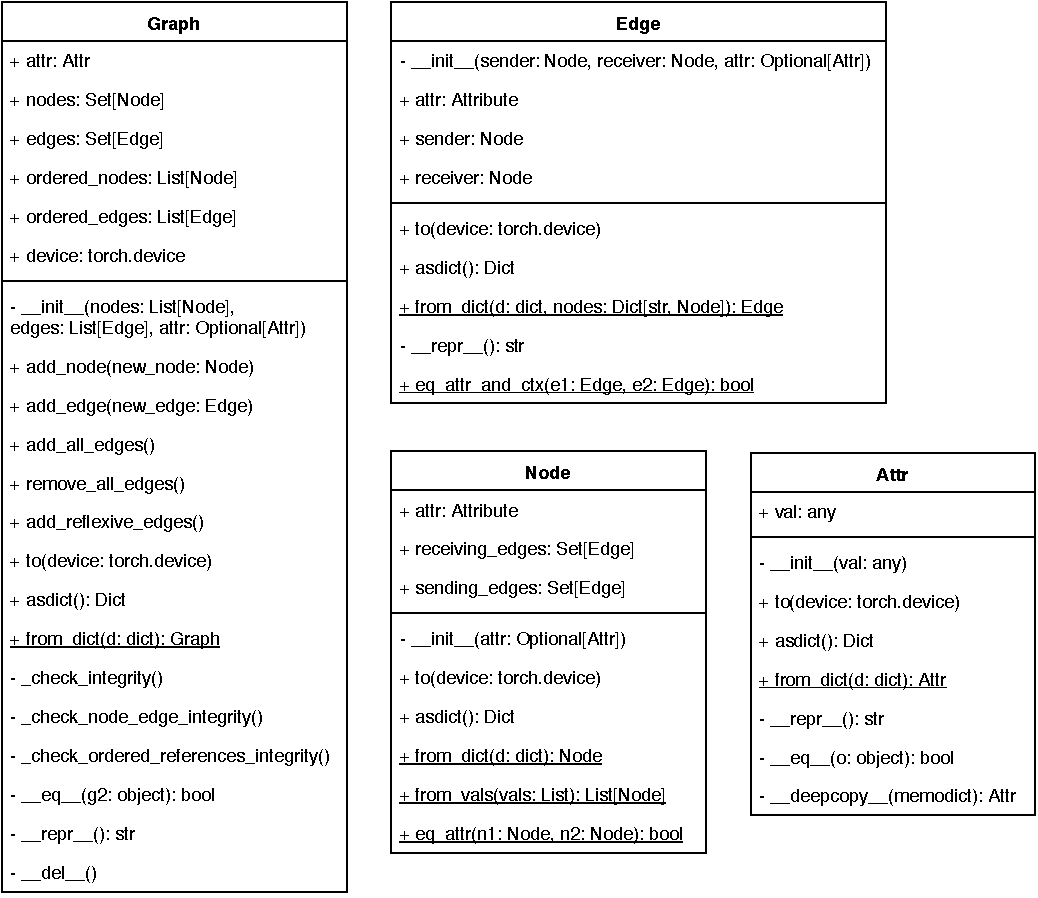
\includegraphics[scale=0.65]{resources/graphnets-datastructs}
    \caption[Class diagram of the graph network library data structure classes]{Class diagram of the graph network library data structure classes, representing a directed, attributed multigraph}\label{fig:classdiagramgndatastructs}
\end{figure}

The graph data structures are four classes, namely \texttt{Graph}, \texttt{Edge}, \texttt{Node}, and \texttt{Attribute}. They are the implementation of a directed, attributed multigraph\footnote{A multigraph is a graph which may have multiple edges (also called parallel edges). For example, there may be two edges pointing from a given node $v_1$ another node $v_2$.} with a global attribute. Figure \ref{fig:classdiagramgndatastructs} depicts the classes with attributes and methods.

The \texttt{Graph} class stores references to all contained nodes and edges. They are stored in a set and in a list for performance reasons: The set allows to determine in $\mathcal{O}(1)$ time whether a node/edge is contained in the graph. The list in turn allows for $\mathcal{O}(n)$ comparison of two isomorphic graphs. The method \texttt{\_check\_integrity()} validates, whether the edges are exclusively connecting nodes contained in the \texttt{nodes} set. It also ensure that the elements contained in \texttt{nodes} and \texttt{ordered\_nodes} are equivalent (and for edges respectively). The \texttt{Graph}'s \texttt{\_\_del\_\_} method is overwritten because it traverses the graph and searches for PyTorch tensors which are placed on the GPU. Upon deletion it moves them to the CPU to ensure their garbage collection after destruction of the \texttt{Graph} object.

An \texttt{Edge} requires two nodes (sender and receiver) to be passed to its constructor. The edge adds itself to the \texttt{receiving\_edges} set of the receiver and \texttt{sending\_edges} set of the sender. \texttt{Edge} objects must therefore be created after \texttt{Node}s.

All three, \texttt{Graph}, \texttt{Node}, and \texttt{Edge} have in common that they have an attribute \texttt{attr} of type \texttt{Attr}. An attribute can hold any value in its \texttt{val} attribute. In the pagerank example, the \texttt{val} of an attribute may for instance be a tuple of screenshots.

\subsubsection{Aggregation and Update Functions}

Aggregation functions serve the purpose of converting a set of attributes into a single attribute. Update functions exist for nodes, edges, and the global state and map their attributes to new, updated attributes. In the graph network framework aggregation functions are denoted by $\rho$ and update functions by $\phi$. All aggregation functions and their relationships can be seen in the class diagram in Figure \ref{fig:classdiagramgnfunctionsaggr}.

\begin{figure}\centering
    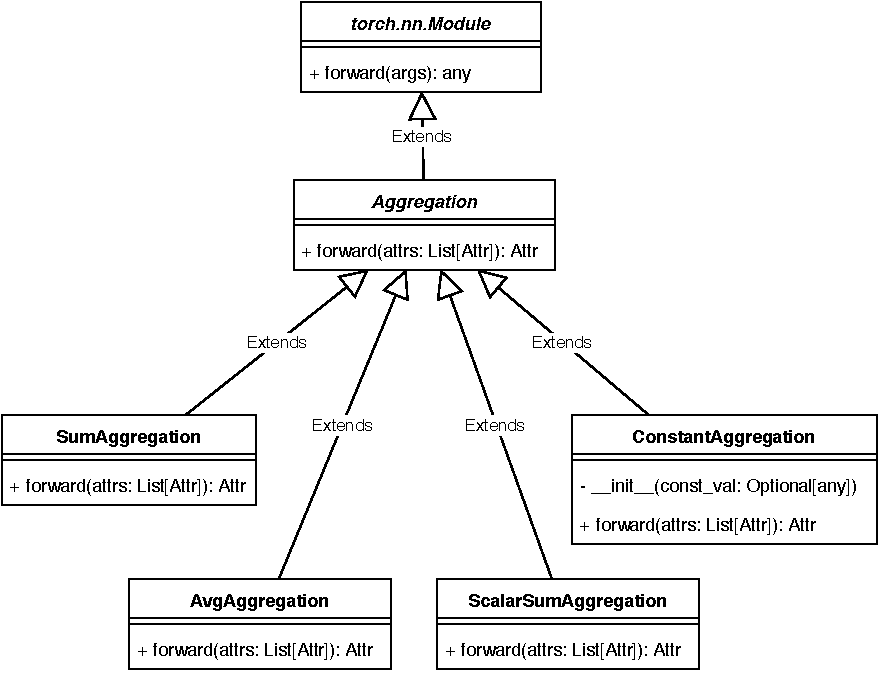
\includegraphics[scale=0.65]{resources/graphnets-functions-aggr}
    \caption{Class diagram of the graph network library aggregation functions}\label{fig:classdiagramgnfunctionsaggr}
\end{figure}

The \texttt{Aggregation} class is abstract and may be implemented by the user of our library. An aggregation can be used for nodes and edges alike. Several common, default implementations are provided, namely

\begin{itemize}
    \item \texttt{SumAggregation}. Sums up the vectors (PyTorch tensor objects) in the set of attributes (parameter \texttt{attrs}) element-wise and returns the resulting vector wrapped in a new \texttt{Attr} object.
    \item \texttt{AvgAggregation}. Works like \texttt{SumAggregation} with subsequent division by the length of \texttt{attrs}.
    \item \texttt{ScalarSumAggregation}. Operates on a list of attributes which hold scalar values, e.g. Python \texttt{float} or \texttt{int} values. It sums them up and returns the resulting value wrapped in a new \texttt{Attr} object.
    \item \texttt{ConstantAggregation}. Ignores the list of attributes entirely and returns a constant value which can be passed to the constructor. This aggregation is useful in a cases where the set of nodes or edges does not contain any useful attributes yet. For instance in the encoder of a GN.
\end{itemize}

The update functions are specific to edges, nodes, and the global state. Therefore, three abstract classes exist, namely \texttt{EdgeUpdate}, \texttt{NodeUpdate}, \texttt{GlobalStateUpdate}, corresponding to $\phi^e$, $\phi^v$, and $\phi^u$, respectively. The classes are abstract because the update may be chosen by the user of the library. The relationships can be seen in the class diagram in Figure \ref{fig:classdiagramgnfunctionsupdate}.

\begin{figure}\centering
    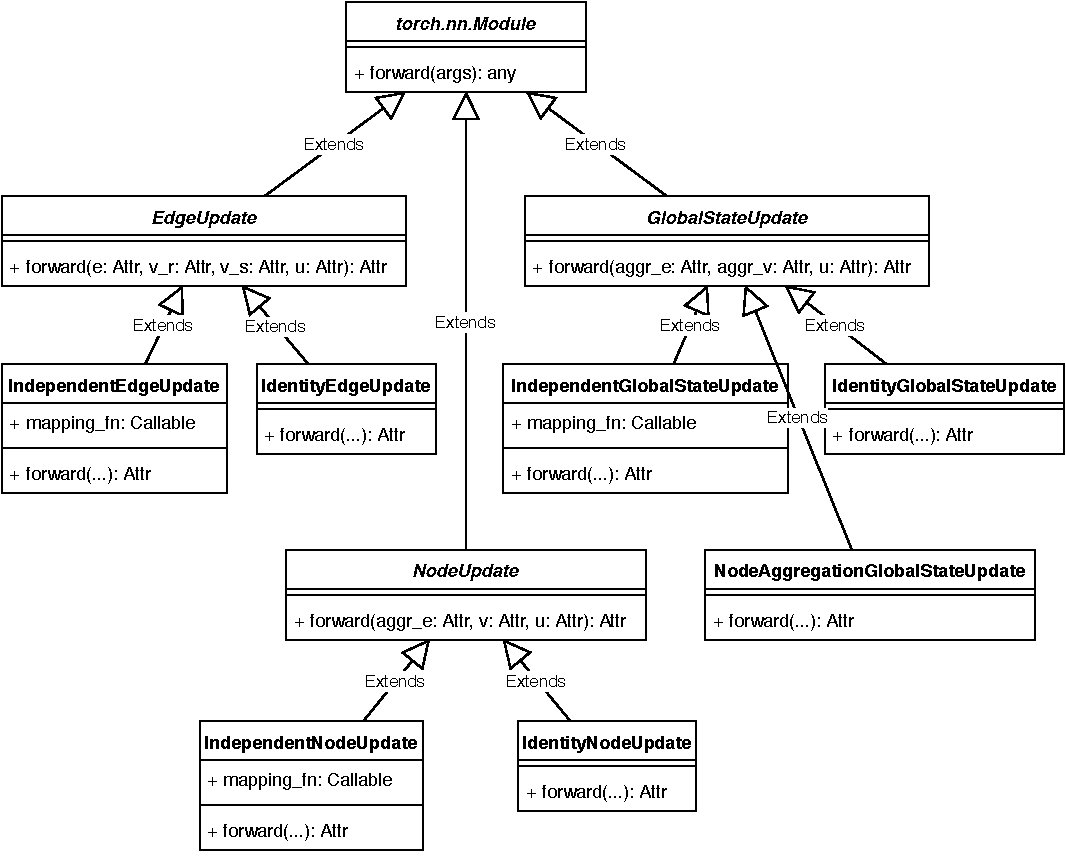
\includegraphics[scale=0.65]{resources/graphnets-functions-update}
    \caption{Class diagram of the graph network library update functions}\label{fig:classdiagramgnfunctionsupdate}
\end{figure}

For all three types of update functions, the library comes with two default implementations: First, the indepdendent update (\texttt{IndependentEdgeUpdate}, \texttt{IndependentNodeUpdate}, \texttt{IndependentGlobalStateUpdate}). An indepdentent update function takes a parameter called \texttt{mapping\_fn}. The result of a forward pass is the application of that mapping function $f_\text{map}$ to the previous edge (or node or global state) attribute. Mathematically that is \begin{align}
\phi^e\left(\bm{e}_k,\bm{v}_{r_k},\bm{v}_{s_k},\bm{u}\right)=&f_\text{map}\left(\bm{e}_k\right)\\
\phi^v\left(\bm{\overline{e}}'_i,\bm{v}_i,\bm{u}\right)=&f_\text{map}\left(\bm{v}_i\right)\\
\phi^u\left(\bm{\overline{e}}',\bm{\overline{v}},\bm{u}\right)=&f_\text{map}\left(\bm{u}\right)\,.
\end{align}Verbally described, everything but the previous attribute value is discarded and the new attribute value is computed with the mapping function.

The identity update functions leave the attribute values unaltered.

\subsubsection{GN Block}

\begin{figure}\centering
    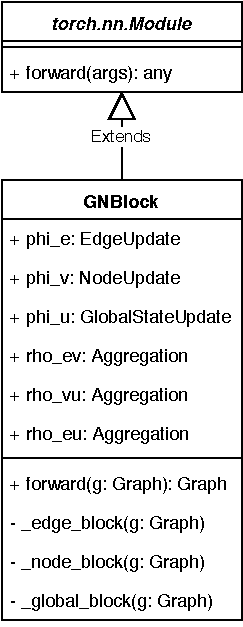
\includegraphics[scale=0.65]{resources/graphnets-block}
    \caption{Class diagram of the graph network library GNBlock class}\label{fig:classdiagramgnblock}
\end{figure}

The GN block is the core component of the library. It inherits from the PyTorch class \texttt{torch.nn.Module} (see class diagram in Figure \ref{fig:classdiagramgnblock}). Its input is a graph and it outputs a transformed version of that graph, by passing it through the \texttt{forward} method. The implementation of \texttt{forward} is exactly matching the flow shown in Figure \ref{fig:fullgraphblock}.

An instantiation of a \texttt{GNBlock} object requires update and aggregation functions. The correspondence between functions and attributes is shown in Table \ref{tab:gnblockattrs}.

\begin{table}
    \centering
    \begin{tabular}{ l l l }
        \hline
        \textbf{Function} & \textbf{Attribute} & \textbf{Default}\\
        \hline
        $\phi^e$ & \texttt{phi\_e} & \texttt{IdentityEdgeUpdate} \\
        $\phi^v$ & \texttt{phi\_v} & \texttt{IdentityNodeUpdate} \\
        $\phi^u$ & \texttt{phi\_u} & \texttt{IdentityGlobalStateUpdate} \\
        $\rho^{e\rightarrow v}$ & \texttt{rho\_ev} & \texttt{ConstantAggregation} \\
        $\rho^{e\rightarrow u}$ & \texttt{rho\_eu} & \texttt{ConstantAggregation} \\
        $\rho^{v\rightarrow u}$ & \texttt{rho\_vu} & \texttt{ConstantAggregation} \\
        \hline
    \end{tabular}
    \caption[Mapping from \texttt{GNBlock} attributes to graph network functions]{Mapping from \texttt{GNBlock} attributes (see class diagram in Figure \ref{fig:classdiagramgnblock}) to graph network functions (described in Section \ref{sec:graphnetworks}). The default value is chosen if the attribute is left unspecified.}
    \label{tab:gnblockattrs}
\end{table}

The GN block simplifies the creation of a GN significantly. After specifying aggregation and update functions, a graph can be passed to a \texttt{GNBlock} instance is is processed by it. Listing \ref{lst:gnblock} shows this flow.

\begin{lstlisting}[
    label={lst:gnblock},
    language=Python,
    caption={Sample usage of the \texttt{GNBlock} class},
    captionpos=b
]
core_block = GNBlock(
    phi_e=CoreEdgeUpdate(drop_p),
    phi_v=CoreNodeUpdate(drop_p),
    phi_u=CoreGlobalStateUpdate(drop_p),
    rho_ev=AvgAggregation(),
    rho_vu=AvgAggregation(),
    rho_eu=AvgAggregation())

g = Graph()
# add attributed nodes and edges to g ...
g_processed = core_block(g)
\end{lstlisting}

\subsubsection{Future Features and Improvements}

The current implementation of the library is processing each graph individually. Batches can not be processed in parallel, which is due to the nature of graphs: A single batch may contain many graphs of different size and shape. A performance boost could be gained by implementing CUDA kernels for the some common update and aggregation functions that handle batches.

A useful feature would be a greater toolbox of implemented update and aggregation functions. Also, composition of GN blocks into actual networks could be simplified with pre-defined modules.

In our current implementation the critical features of the components are being unit tested. There is also an end-to-end test which trains a GN to learn the identity function, thereby ensuring PyTorch's automatic differentiation works through GN blocks. Before performing a greater refactoring (e.g. the implementation of CUDA kernels), a higher test coverage would be desirable.
